\subsection{ダイオードの特性実験}
\subsubsection{ダイオードの実験器具}
使用した実験器具を\wtab{kigu}に示す.
\begin{table}[h]
  \centering
  \caption{実験装置}
  \label{tab:kigu}
  \scalebox{1.0}{
  \begin{tabular}{cccccc}
    \hline
    機器名&製造元&型番&シリアル番号(または管理番号)\\
    \hline
    ダイオード&不明&1N4002&不明\\
    直流電源&YOKOGAWA&PA1811&L96-000668\\
    直流用電圧計&YOKOGAWA&YAS 1991&71 BA0 3371\\
    ミリアンペア直流用電流計&YOKOGAWA&YES 1990&70 BA0 1812\\
    マイクロアンペア直流用電流計&YOKOGAWA&B-5036.H1.10/10&B5036\\
    \hline
  \end{tabular}
}
\end{table}

\subsubsection{ダイオードの実験方法}
\begin{enumerate}[(1)]
	\item \wfig{bias}のように回路を構築した.なお,ダイオード$D$は1N4002を用いた.
	\item 順バイアス$E$を加え,電圧$V_{D}$(0から0.8\,\rm{V}まで0.1\,\rm{V}刻みで変化)と電流$I_{D}$を計測した.その際,電流計はミリアンペア計を利用し,端子は$300\,\rm{mA}$に接続した.
	\item 計測したデータをプロットし,データ数が不足していた$0.6\,\rm{V}$から$0.8\,\rm{V}$の区間は$V_{D}$を$0.025\,\rm{V}$刻みで計測した.
	\item 計測データを基に,$V_{D}-I_{D}$特性をグラフにまとめた.
	\item 回路を\wfig{bias}の回路でダイオード$D$を逆向きに接続するように変更し,逆バイアス$E$を$0\,\rm{V}$から$0.8\,\rm{V}$まで$1\,\rm{V}$刻みで加え,電流$V_{D}$と電流$I_{D}$を計測した.なお,電流はマイクロアンペア計で計測し,端子は$3\,\rm{mA}$に接続した.
	\item 順バイアスと同様に,$V_{D}-I_{D}$特性をグラフにまとめた.
	\begin{figure}[h]
	\centering
	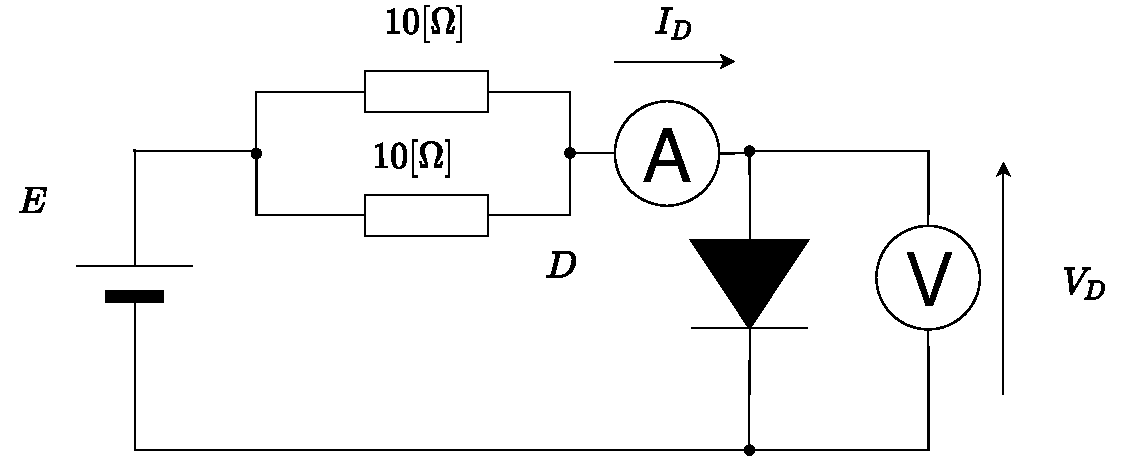
\includegraphics[scale=0.65]{./fig/bias.pdf}
	\caption{順バイアス測定回路}
	\label{fig:bias}
	\end{figure}
\end{enumerate}

\subsubsection{ダイオードの結果}
\begin{itemize}
	\item 測定結果を\wtab{bias}に示す.$0.400\,\rm{V}$まではほぼ電流が流れなかったが,それ以降は電圧増加とともに電流も増加し,$0.650\,\rm{V}$付近から急激に増加していることがわかる.
このような変化は抵抗の変化の仕方と異なっている.
	\item 順バイアスを印加した際の計測データから作成したグラフを近似曲線とともに\wfig{vias-graph-n}に示す.
	\item 逆バイアスを印加した際のグラフを\wfig{bias-rev}に示す.
	\begin{table}[h]
	\centering
	\caption{順・逆バイアスにおける電圧電流の関係}
	\label{tab:bias}
	\scalebox{1.0}{
	\begin{tabular}{cccc}
	\hline
	電圧(順バイアス)$V_{D}$[\rm{V}]  &電流$I_{D}$[\rm{mA}]   & 電圧(逆バイアス)$V_{D}$[\rm{V}] &  電流$I_{D}$[$\mu$\rm{A}] \\
	\hline
	0.000 & 0.0   & 0 & 0 \\
	0.100 & 0.0   & 1 & 0 \\
	0.200 & 0.0   & 2 & 0 \\
	0.300 & 0.0   & 3 & 0 \\
	0.400 & 0.0   & 4 & 0 \\
	0.500 & 1.0   & 5 & 0 \\
	0.600 & 2.0   & 6 & 0 \\
	0.625 & 4.0   & 7 & 0 \\
	0.650 & 6.0   & 8 & 0 \\
	0.675 & 10.0  &  - &  - \\
	0.700 & 19.8  &  - &  - \\
	0.725 & 29.0  & -  & -  \\
	0.750 & 48.0  & -  & -  \\
	0.775 & 71.0  & -  &  - \\
	0.800 & 116.0 & -  &-  \\
	\hline
	\end{tabular}
	}
\end{table}

\begin{figure}[h]
\centering
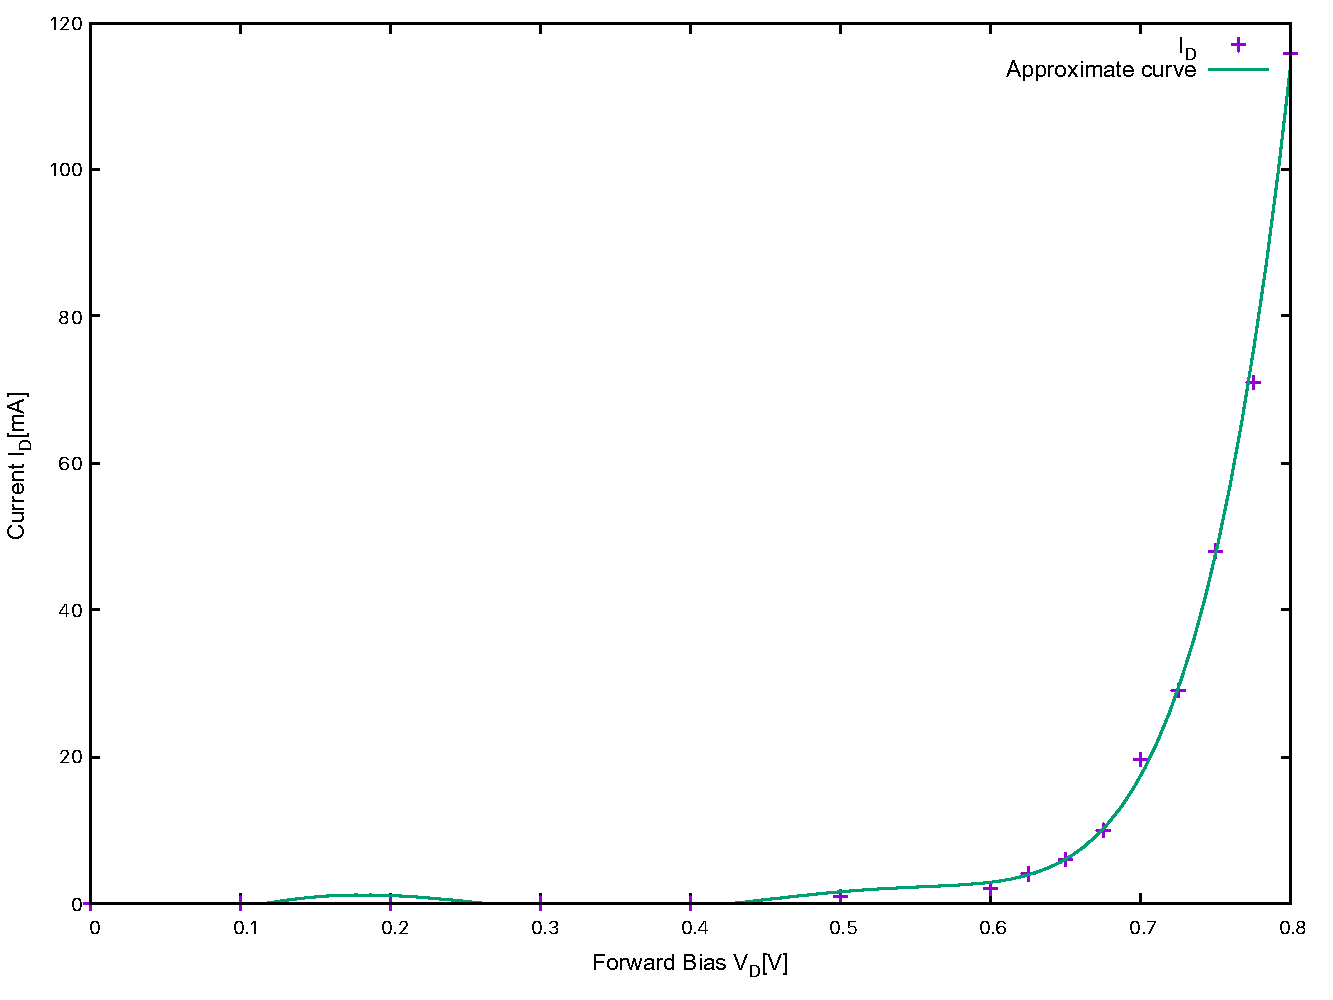
\includegraphics[scale=0.65]{./data/diode/bias-n.pdf}
\caption{順バイアスの$V_{D}-I_{D}$特性}
\label{fig:vias-graph-n}
\end{figure}
\end{itemize}

\begin{figure}[h]
\centering
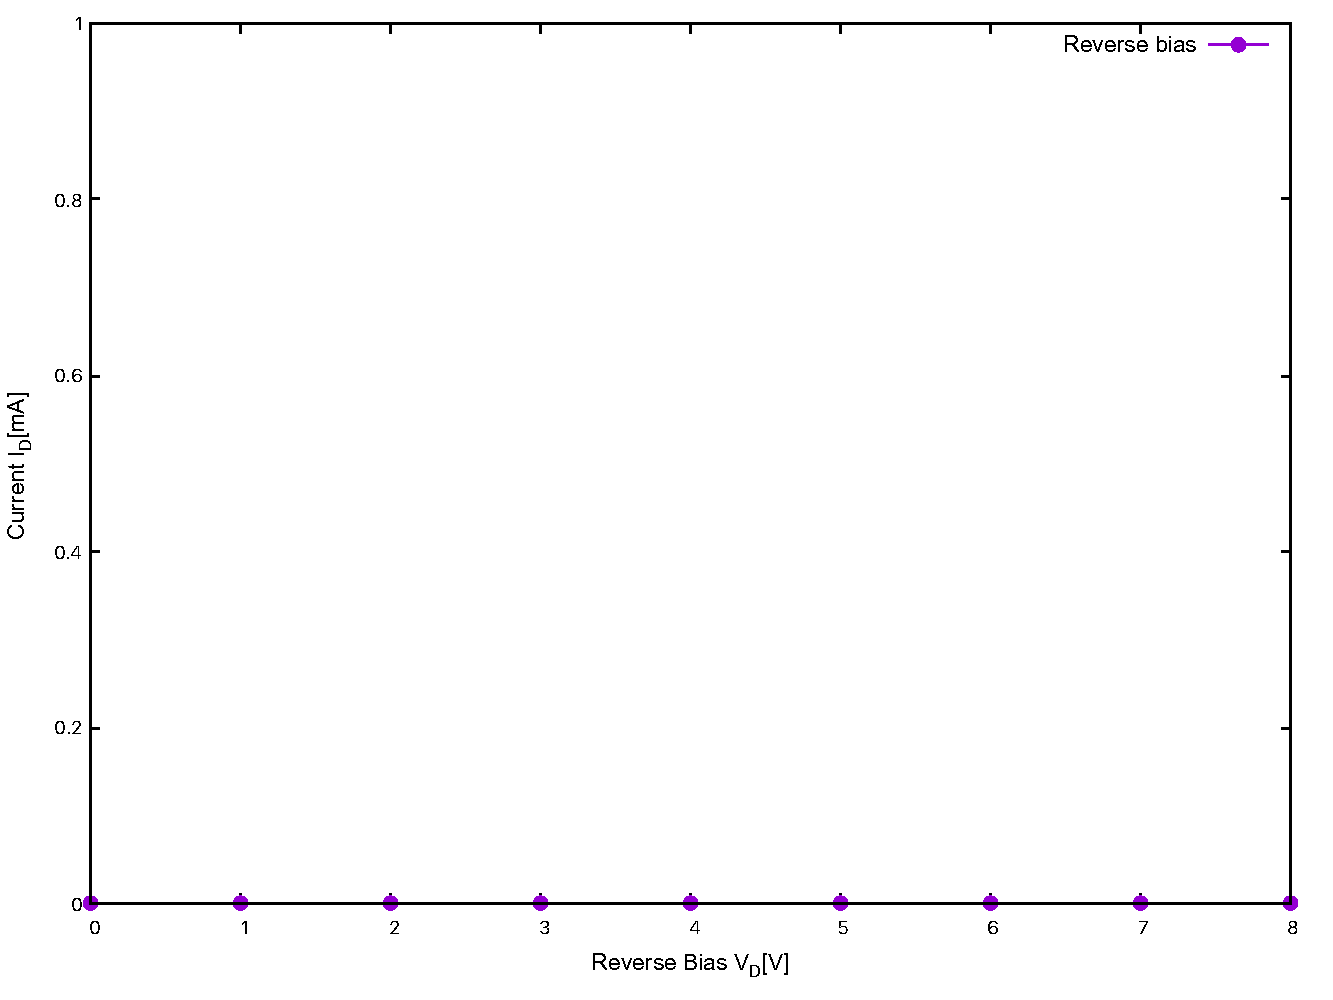
\includegraphics[scale=0.65]{./data/diode/bias-rev.pdf}
\caption{逆バイアスの$V_{D}-I_{D}$特性}
\label{fig:bias-rev}
\end{figure}

\clearpage
\subsubsection{ダイオードの考察}
\begin{enumerate}[(1)]
\item 直流電圧電流特性グラフを説明せよ.(立ち上がり電圧$V_{J}$をグラフに書き込む.また,$E=0.8\,\rm{V}$としたときの負荷線を描き,動作点Pの微分抵抗$r_{d}=\Delta V_{D}/\Delta I_{D}$を求めよ.$r_{d}$,$V_{J}$,理想ダイオードからなる等価回路を描き,どの部分がどのような特性を表しているのか説明せよ)

\wfig{vias-graph-n}に$V_{J}$,負荷線,を加えたグラフを\wfig{vias-graph-n-1}に示す.
また,各特性値の導出方法を\wtab{how}にまとめる.

\begin{table}[h]
\centering
\caption{特性値の導出方法}
\label{tab:how}
\scalebox{0.8}{
\begin{tabular}{cl}
\hline
特性値    & 導出方法  \\
\hline
動作点$P$ &負荷線の式(\weq{IF})に電圧$V_{D}$を代入した$I_{D}'$と計測電流$I_{D}$の誤差が最も少ない点($0.7\,\rm{V}$, $19.8\,\rm{mA}$)とした.(\wtab{PT}) \\
接線    & 動作点$P$を中間点とするような$(0.675\,\rm{V}, 10\,\rm{mA})$と$(0.725\,\rm{V}, 29\,\rm{mA})$を変位として\weq{int}のように導出 \\
$V_J$   & 接線と$x$軸との交点を通る$y$軸に並行な直線とした.(\weq{vj}) \\
負荷線   & \weq{IF}のように合成抵抗と電圧値により導出\cite{1130282271098203264}.\\
微分抵抗$r_d$ & 動作点$P$を中間点とするような$(0.675\,\rm{V}, 10\,\rm{mA})$と$(0.725\,\rm{V}, 29\,\rm{mA})$を変位として\weq{rd}のように算出\\
\hline
\end{tabular}
}
\end{table}

\begin{align}
\centering
I_{D}&=\frac{\Delta I_{D}}{\Delta V_{D}} V_{D} +V_{J}\nonumber \\
\frac{\Delta I_{D}}{\Delta V_{D}} &=\frac{(29-10)\times 10^{-3}}{0.725-0.675}=380\times 10^{-3}\,\rm{S}\nonumber \\
V_{J}&=I_{D}-\frac{\Delta I_{D}}{\Delta V_{D}} V_{D}\nonumber \\
この&接線は動作点を通るので\nonumber \\
&=19.8\times 10^{-3}-380\times 10^{-3}\cdot 0.7=-246.2\,\rm{mV}\nonumber \\
\therefore I_{D}&=380V_{D} -246.2[\rm{mA}]\label{eq:int}
\end{align}
\begin{align}
\centering
V_{J}の座標&は接線でI_{D}=0となる点であるから\weq{int}より\nonumber \\
0&=380V_{J} -246.2\nonumber \\
246.2&=380V_{J}\nonumber \\
\therefore V_{J}& \fallingdotseq 0.65\,\rm{V} \label{eq:vj}
\end{align}
\begin{align}
\centering
R&=\frac{10\cdot10}{10+10}\nonumber \\
&=5\,\rm{\Omega}\nonumber \\
I_{D}&=-\frac{1}{R}V_{D}+\frac{E}{R}\nonumber \\
&=-\frac{1}{5}V_{D}+\frac{0.8}{5}\,\rm{A}\nonumber \\
&=\left(-\frac{1}{5}V_{D}+\frac{0.8}{5}\right)\times 10^{3}[\rm{mA}]
\label{eq:IF}
\end{align}

\begin{table}[h]
\centering
\caption{動作点$P$の導出}
\label{tab:PT}
\scalebox{1.0}{
\begin{tabular}{cccc}
\hline
電圧$V_{D}$[\rm{V}]  &計測電流$I_{D}$[\rm{mA}]   & 算出した$I_{D}'$[\rm{mA}] & 誤差$|I_{D}-I_{D}'|$[\rm{mA}] \\
\hline
0.000 & 0.0   & 160 & 160 \\
0.100 & 0.0   & 140 & 140 \\
0.200 & 0.0   & 120 & 120 \\
0.300 & 0.0   & 100 & 100 \\
0.400 & 0.0   & 80  & 80  \\
0.500 & 1.0   & 60  & 59  \\
0.600 & 2.0   & 40  & 38  \\
0.625 & 4.0   & 35  & 31  \\
0.650 & 6.0   & 30  & 24  \\
0.675 & 10.0  & 25  & 15  \\
0.700 & 19.8  & 20  & 0.2 \\
0.725 & 29.0  & 15  & 14  \\
0.750 & 48.0  & 10  & 38  \\
0.775 & 71.0  & 5   & 66  \\
0.800 & 116.0 & 0   & 116 \\
\hline
\end{tabular}
}
\end{table}

\begin{figure}[h]
\centering
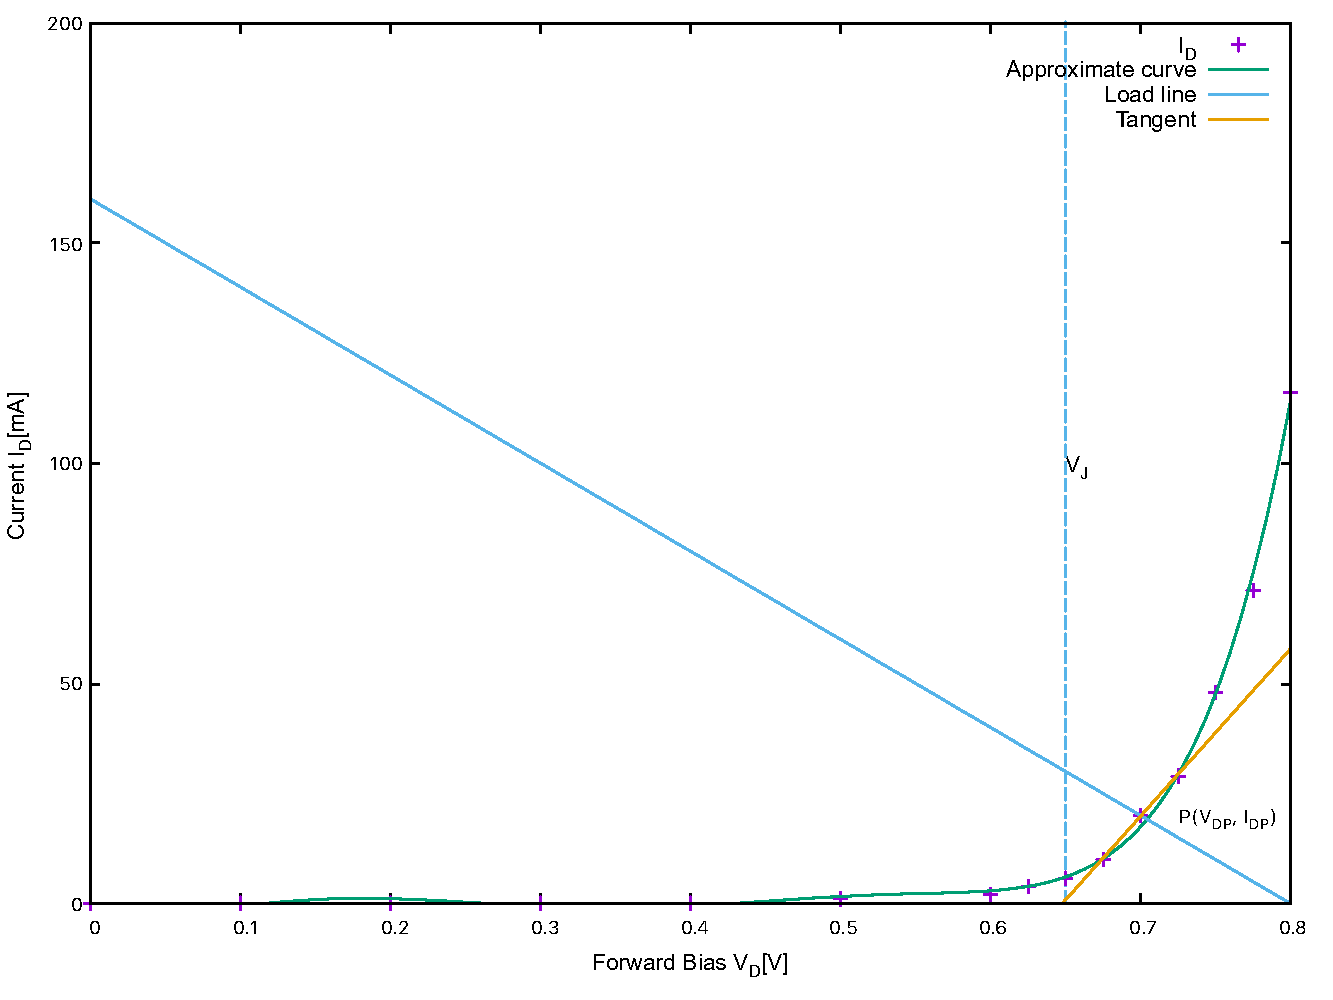
\includegraphics[scale=0.65]{./data/diode/bias-n-1.pdf}
\caption{順バイアスにおける負荷線と$V_{J}$}
\label{fig:vias-graph-n-1}
\end{figure}
\begin{align}
r_{d}&=\frac{\Delta V_{D}}{\Delta I_{D}}\nonumber \\
&=\frac{0.725-0.675}{(29.0-10.0)\times 10^{-3}}\nonumber \\
&=\frac{0.05}{19.0\times 10^{-3}}\nonumber \\
& \fallingdotseq 2.63\,\rm{\Omega}
\label{eq:rd}
\end{align}

理想ダイオードからなる等価回路は\wfig{eqc}となる~\cite{adsfcaw}.
$V_{J}$はダイオードの内部で発生する電界から生まれる電圧降下を示し,
$r_{d}$は動作点近傍でのダイオードの抵抗を表す~\cite{sdfvadfcdf}.
理想ダイオードは実際のダイオードと異なり,順方向にバイアスされているまたは,端子電圧が$0\,\rm{V}$の際に完全な導体として振る舞い,逆バイアスが印加されている時に完全な絶縁体となるものである.これらがダイオードの整流作用を起こしている~\cite{adsfcaw}.
	\begin{figure}[h]
	\centering
	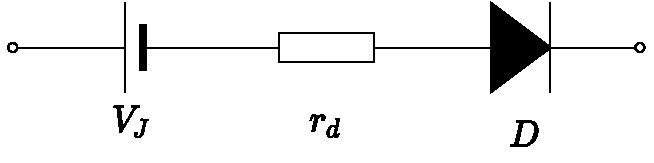
\includegraphics[scale=0.5]{./fig/eqc.pdf}
	\caption{理想ダイオードからなる等価回路}
	\label{fig:eqc}
	\end{figure}

	\item 実験で用いたダイオードのデータシートから逆方向電流の値を調べよ.また,逆バイアスの場合でもわずかに電流が流れる理由を図を用いて説明せよ.(多数キャリアや少数キャリアという観点から考えること。\wfig{fig2}を用いるとよい.)

データシート~\cite{sdfgvhsd}より逆電流$I_{R}$は$25^{\circ}$Cで最大$10\,\rm{\mu A}$流れることがわかる.
逆バイアスを印加した際,接合面で多数キャリアが再結合で減少する.
また\wfig{fig2}ではp型において,多数キャリアのみに注目しているため,電子が移動せず,電流が流れないように考えられるが,実際は少数キャリアである電子が移動する(ドリフト)ためわずかに電流が流れてしまう.
\end{enumerate}
